\documentclass[10pt]{beamer}

\usetheme[progressbar=frametitle, numbering=fraction,]{metropolis}
\setbeamertemplate{footnote}{%
  \parindent 0em\noindent%
  \raggedleft%\raggedright
  \usebeamercolor{footnote}\hbox to 0.8em{\hfil\insertfootnotemark}\insertfootnotetext\par%
}

\renewcommand{\footnoterule}{%
\kern -3pt
\hrule width \textwidth height 0pt
\kern 3pt
}


\usepackage{booktabs}
\usepackage{pgfplots}
\usepgfplotslibrary{dateplot}
\usepackage{texshade}      
\usepackage{amsmath}
\usepackage{amssymb}
\usepackage{xspace}
\usepackage{xcolor}
\usepackage{appendixnumberbeamer}
\usepackage{multirow}

\newcommand{\themename}{\textbf{\textsc{metropolis}}\xspace}

\title{Simpson's Paradox}
\subtitle{It's sometimes not about the bigger picture}
\date{\today}
\author{Saket Choudhary}
\institute{}
%\titlegraphic{\hfill
\includegraphics[height=1.5cm]{logo}}

\begin{document}

\maketitle

\begin{frame}[fragile]{Yule-Simpson Effect: Example from University Admission}
\footnotesize
 %\begin{columns}[T,onlytextwidth]
    %\column{0.3\textwidth}
    \begin{center}
    \begin{table}
    \begin{tabular}{|c|c|c|}
    \hline
    & Female & Male\\
    \hline
    Applicants & 550 & 550 \\
    \hline 
    Admitted & 28.2\% & 41.8\% \\
    \hline
    \end{tabular}
    \caption{Acceptance percentage of female candidates is far less}
    \end{table}
    \end{center}
    \begin{center}
	\uncover<2->{\footnotesize
    \begin{table}
\begin{tabular}{|c|c|c|c|c|}
\hline
\multirow{3}{*}{} & \multicolumn{2}{|c|}{Female} &  \multicolumn{2}{|c|}{Male}\\
\cline{2-5}
& Applicants & Admitted & Applicants & Admitted\\
\cline{2-5}
Department A & 150 & 50\% & 400 & 50\%\\
\hline
Department B & 400 & 20\% & 150 & 20\%\\
\cline{1-5}
\end{tabular}
\caption{Departments do not display gender specific bias. Lower admission rates in female arises due females applying to department which are `harder' to get into}
\end{table}
    }
    \end{center}
\end{frame}

\begin{frame}[fragile]{Yule Simpson Effect: Single Cells}
\footnotesize\let\thefootnote\relax{Maamar, Hédia, et al. Genes \& development, 2013}

\begin{figure}
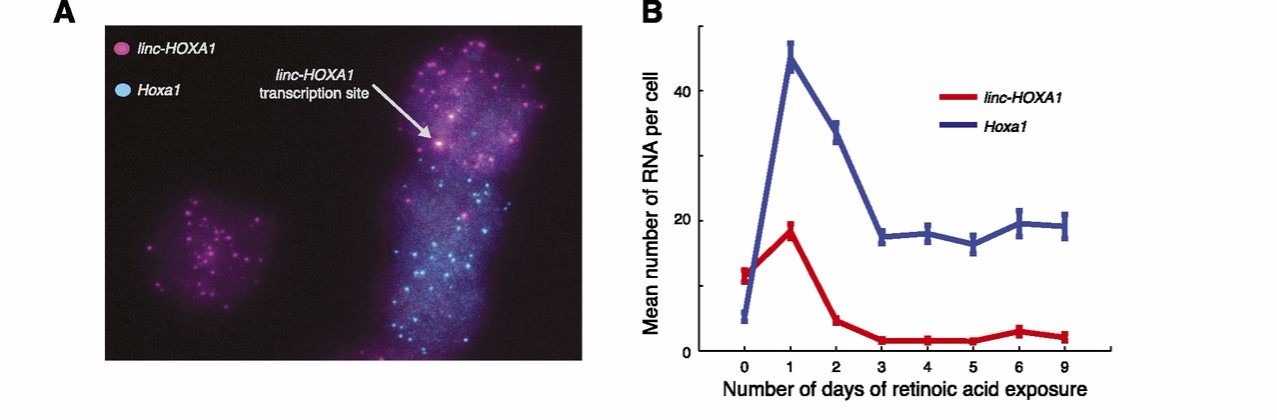
\includegraphics[scale=0.23]{HOXA1-bulk}
\end{figure}
\uncover<2->{
\begin{figure}
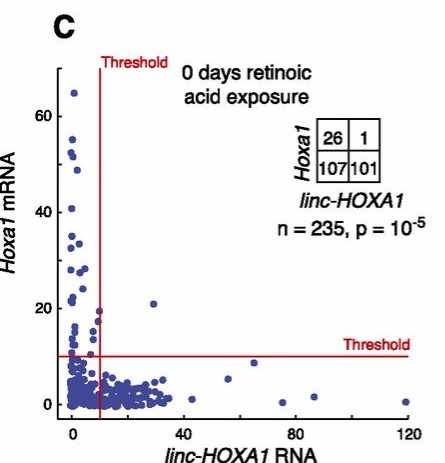
\includegraphics[scale=0.25]{HOXA1-single}
\end{figure}
}

\end{frame}



\end{document}
